%!TEX root = ../../main.tex

\chapter{Data Preprocessing}

Based on \cite{football-predictor} five sliding windows for match data were implemented. The idea of these sliding windows is to deliver match data in historical order and to aggregate data on a team's performance during the last 10 games.
First the relevant data was extracted in chronological order with the following SQL statement:

\begin{lstlisting}[language=SQL, caption=SQL code for Sliding Window]
SELECT id, country_id, league_id, season, date, home_team_api_id, away_team_api_id, home_team_goal, away_team_goal, B365H, B365D, B365A, shoton, shotoff, possession
FROM Match
ORDER BY date asc
\end{lstlisting}

Since the bookkeeper odds are highly correlated, as has been pointed out in \autoref{chap:data_understanding}, only Bet365 data (B365H = odds home team wins, B365A = odds away team wins, B365D = odds draw) will be used.


\section {Slliding Windows or Data Options}
This part defines five different sliding windows which are used to predict the final results and the scored goals.
\subsection {Option 1}
For the first sliding window or option, data on shoton, shotoff and possession are not necessary and therefore are dropped. Moreover, rows without odds are dropped as well. The resulting data is saved as a CSV file:


\begin{lstlisting}[language=Python, caption=Python code for matches\_all.csv]
conn = sqlite3.connect("../data/eusoccerdatabase.sqlite")
query = "SELECT id, country_id, league_id, season, date, match_api_id, home_team_api_id, away_team_api_id, home_team_goal, away_team_goal, B365H, B365D, B365A, shoton, shotoff, possession FROM Match ORDER BY date asc"
df = pd.read_sql_query(query, conn)
df = df[np.isfinite(df['B365H'])] # drop rows without odds
df_noxml=df.drop(['shoton', 'shotoff', 'possession'], axis=1)
df_noxml.to_csv("../data/matches_all.csv")
\end{lstlisting}

This CSV file consists now of 22592 rows each representing one football match including information on how many goals each team scored, what the odds were and the date of the match:

\begin{figure}[H]
\begin{center}
\includegraphics[scale=.55]{matches_all_csv.png}
\end{center}
\caption{Data for Option 1}
\label{fig:matches_all_csv}
\end{figure}


This CSV file was then used for the first sliding window. The code for it \cite{sliding01} expects a CSV file and processes it row by row. For every match the outcome of the game based on scored goals is calculated. Moreover, statistics on how each of the two opponents performed in the previous ten games are generated:

\begin{figure}[H]
\begin{center}
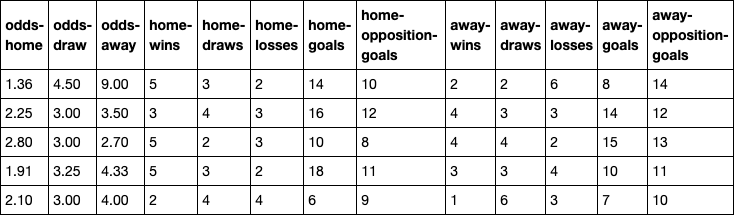
\includegraphics[scale=.55]{sliding_window_option1.png}
\end{center}
\caption{Sliding Window Option 1}
\label{fig:sliding_window_option1}
\end{figure}


\subsection {Option 2}
This option, which uses a slightly enhanced version \cite{sliding02} of the first sliding window code, adds statistics on goal shots:

\begin{figure}[H]
\begin{center}
\includegraphics[scale=.55]{sliding_window_option2.png}
\end{center}
\caption{Sliding Window Option 2}
\label{fig:sliding_window_option2}
\end{figure}

Unfortunately due to the poor choice of data origin this option reduces the dataset to 7033 rows. But on the bright site, this option extends the number of features to 21.

\subsection {Option 3}
Based on option 2, option 3 additionally calculates shot accuracy statistics with code written and executed in a Jupyter Notebook \cite{jupyter_sliding}:

\begin{figure}[H]
\begin{center}
\includegraphics[scale=.55]{sliding_window_option3.png}
\end{center}
\caption{Sliding Window Option 3}
\label{fig:sliding_window_option3}
\end{figure}



Option 3 has 29 features and 7033 rows. "x\_shot\_accuracy" represents the percentage of the shots which actually hit the goal or goal keeper and "x\_shot\_efficiency" the percentage of the shots which actually were counted as goals.


\subsection {Option 4}

Option 4 again uses an enhanced enhanced version \cite{sliding04} of the first sliding window code and extends option 2 with ball possession statistics:

\begin{figure}[H]
\begin{center}
\includegraphics[scale=.55]{sliding_window_option4.png}
\end{center}
\caption{Sliding Window Option 4}
\label{fig:sliding_window_option4}
\end{figure}

Ball possession is provided in minutes. This option has 6996 rows and 25 features.

\subsection {Option 5}
The last option is based on option 3 and additionally includes ball possession statistics. It has the highest number of features (33) and 6996 rows. The Python code for it can be found in the same Jupyter Notebook as for option 3 \cite{jupyter_sliding}.


\section {Data Profiling Part 2}

Using Pandas Profiling all sliding windows or options were profiled again. Here is and excerpt of the profile for option 3:

\begin{figure}[H]
\begin{center}
\includegraphics[scale=.6]{profiling_option3.png}
\end{center}
\caption{Pandas Profiling Sliding Window 3}
\label{fig:profiling_option3}
\end{figure}

All features/columns are numerical and no values (cells) are missing. As expected x-shots and x-shots\_on\_target are highly 
correlated. Interestingly zero values are marked as warnings. However, in this context they are fine and still usable. Without having domain knowledge and purely relying on tools, one might be inclined to drop these values and lose valuable information. Another interesting information found in Pandas profiles is the total size in memory. 1.8 MiB shows that the data for option 3 is little and definitely small enough to fit into RAM or GPU memory. This information is valuable, as will be shown later.
\newline
Since the profiles for the other options are similar to the one described above, they will not be explained.


\section {Prediction of the final result}

The prediction of the final result is based on 3 distinguishable classes (H = home team wins, A = away team wins, D = draw).

In the following example, we can see in row 0 that the home team won, which is indicated by a capital "H". The odds that the home team wins were 3.50, 3.30 for a draw and odds of 2.10 that the away team wins. In the last 10 matches the home team won 1 time, finished 3 matches with a draw, lost 6 times and scored 11 goals. Opposing teams were able to win 10 games. Subsequent columns contain the equivalent statistics for the opposing/away team. The second sliding window reduces the total dataset to 7033 rows and generates 21 features.


\begin{figure}[H]
\begin{center}
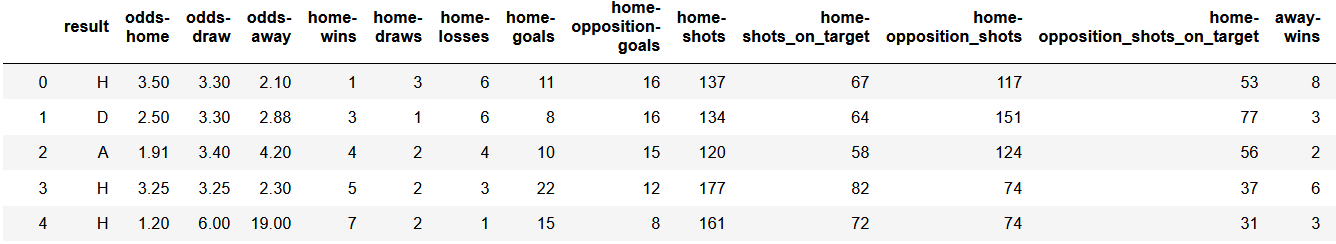
\includegraphics[scale=.55]{results_sliding_window_option2.png}
\end{center}
\caption{Results Sliding Window Option 2}
\label{fig:results_sliding_window_option2}
\end{figure}

The last part of the data preparation is to normalize the dataset by rescaling it to make all the elements lie between 0 and 1 thus bringing all the values of numeric columns in the dataset to a common scale. Almost all ML algorithm requires data in numerical form. For that, we'll go through the encoding methods that are necessary for the machine to interpret the data(more specifically categorical data) and learn from it.

\subsection {Normalization}
Since the input data varies in scale it has to be normalized, except the "result" column which has to be encoded. Normalization is the process which normalizes all input data avoiding negative effects in regards to decisions of a neuron. 
The following lines of code normalize the data in a dataframe:

\begin{lstlisting}[language=Python, caption=Python code for normalization]
from sklearn import preprocessing

column_names_to_not_normalize = ['result']
column_names_to_normalize = [x for x in list(dataframe) if x not in column_names_to_not_normalize ]
x = dataframe[column_names_to_normalize].values
x_scaled = preprocessing.normalize(x)
df_temp = pd.DataFrame(x_scaled, columns=column_names_to_normalize, index = dataframe.index)
dataframe[column_names_to_normalize] = df_temp
\end{lstlisting}



\subsection {Encoding}

The classes H,A,D respectively the outcome of football match which shall be predicted, have to be encoded before they can be used. Using sklearn this can be achieved with only a few lines of code:

\begin{lstlisting}[language=Python, caption=Python code for encoding classes]
from sklearn import preprocessing

le = preprocessing.LabelEncoder()
le.fit([ "H", "A", "D"])
dataframe.loc[:,['result']]=le.transform(dataframe['result'])
\end{lstlisting}



\section {Prediction of the scored goals}

This part differs from the previous one by changing the "result" column to two columns: "home\_team\_goal" and "away\_team\_goal". It means, we are not predicting the winner or draw but we predict the final scored goals. The scored goals are between 0 and 10 for each team.


The following fig. shows the number of goals scored by each team in a game, we can see in row 0 that the home team scored 2 goals and the away team scored 1 goal. The features are based on the last 10 matches as described in the previous sections.


\begin{figure}[H]
\begin{center}
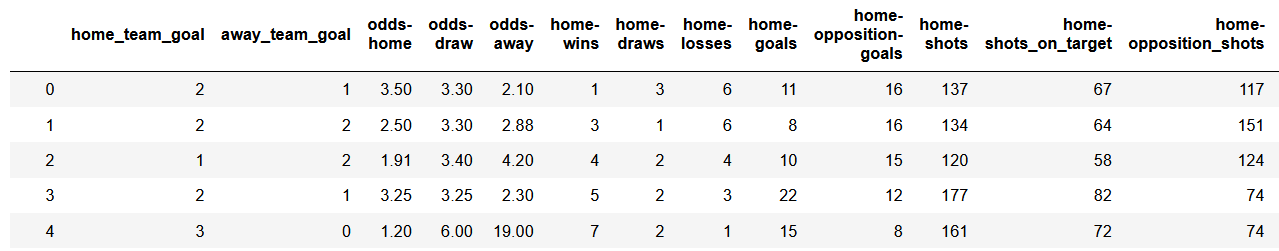
\includegraphics[scale=.55]{goals_sliding_window_option2.png}
\end{center}
\caption{Scored Goals Sliding Window Option 2}
\label{fig:scored_sliding_window_option2}
\end{figure}

The next parts describe the standardization and encoding processes.


\subsection {Normalization}
The goal of normalization is to change the values of numeric columns in the dataset to a common scale, without distorting differences in the ranges of values. The normalization is restricted to the input features and not output features.

Since the input data varies in scale it has to be normalized, except the "home\_team\_goal" and "away\_team\_goal" columns which have to be encoded.
The following lines of code normalize the data in a dataframe:

\begin{lstlisting}[language=Python, caption=Scored goals Python code for normalization]
from sklearn import preprocessing

column_names_to_not_normalize = ['home_team_goal','away_team_goal']
column_names_to_normalize = [x for x in list(dataframe) if x not in column_names_to_not_normalize ]
x = dataframe[column_names_to_normalize].values
x_scaled = preprocessing.normalize(x)
df_temp = pd.DataFrame(x_scaled, columns=column_names_to_normalize, index = dataframe.index)
dataframe[column_names_to_normalize] = df_temp
\end{lstlisting}


\subsection {Encoding}

The goals scored initially are between 0 and 10.
To facilitate prediction before starting encoding, we have reduced the maximum number of goals scored in order to reduce the classes. The following figure shows that choosing to have 5 as the maximum number is a good idea because we have a very small number of rows for 6,7,8,9 and 10 goals scored compared to the others.

\begin{figure}[H]
\begin{center}
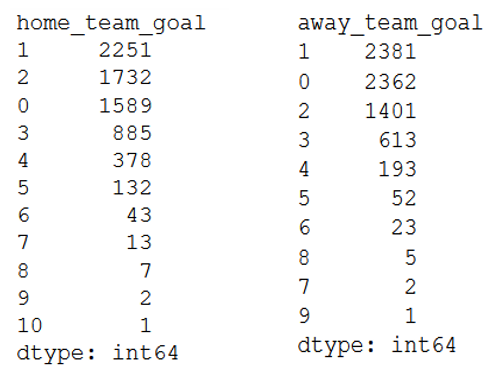
\includegraphics[scale=.6]{goals_counts.png}
\end{center}
\caption{The initial number of rows per each scored goal(s)}
\label{figure:goals_counts}
\end{figure}


The second step is to encode 0 goals to -1, 1 goal tp -0.6, 2 goals to -0.2, 3 goals to 0.2, 4 goals to 0.6 and 5 or more goals to 1.
The following figure \autoref{figure:dataPrep} describes the encoding step.\newline
\begin{figure}[H]
\begin{center}
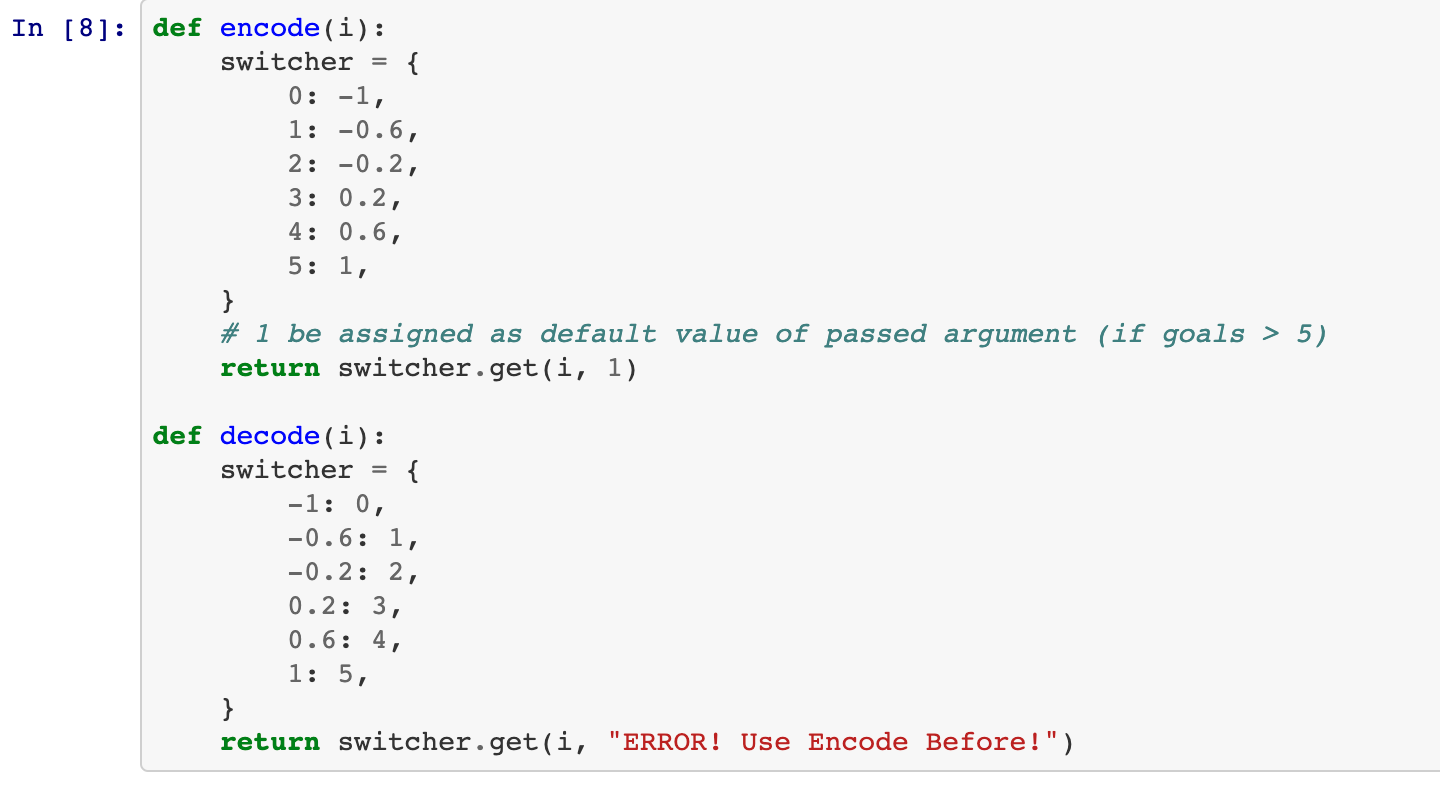
\includegraphics[scale=.6]{datapreprocessing_regression.png}
\end{center}
\caption{Encode and Decode functions}
\label{figure:dataPrep}
\end{figure}



The encode function can be used with the following lines of code:

\begin{lstlisting}[language=Python, caption=Scored goals Python code for encoding classes]
dataframe['home_team_goal'] = dataframe.apply(lambda row: encode(row['home_team_goal']), axis=1)
dataframe['away_team_goal'] = dataframe.apply(lambda row: encode(row['away_team_goal']), axis=1)
\end{lstlisting}


After executing the encode function, we have the following result.

\begin{figure}[H]
\begin{center}
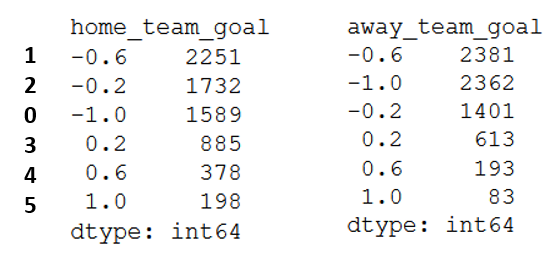
\includegraphics[scale=.6]{encoded_val.png}
\end{center}
\caption{Encoding results}
\label{figure:encoding}
\end{figure}


The decoding function is useful after executing the encoding function in order to have the real scored goals but it keeps predicting 5 as the maximum scored goals (not 10 as it was).



\section {Functions and Input Data For Neural Networks}
The repetitive data preparation tasks encoding, normalization, splitting data into training and test data as well as getting data and prediction labels have been solved using Python functions. Furthermore, Pandas dataframes cannot be used as input for neural networks written with Tensorflow and Keras. The complete code, which has been partly described above, can be found here \cite{colab_nn}.
\newline
Since the data for all options is very little and fits completely into RAM, as has been described above, no input functions for Tensorflow models, e.g. neural networks, had to be written. An excerpt of how the final input data as numpy array for the neural networks described in \autoref{cha:Modelling} looks like can be seen here:

\begin{figure}[H]
\begin{center}
\includegraphics[scale=.6]{input_data.png}
\end{center}
\caption{Excerpt of Input Data for Neural Networks as Numpy Array}
\label{fig:inpud_data}
\end{figure}














